\documentclass[notes, ignorenonframetext, compress, 9pt, xcolor=svgnames, aspectratio=169]{beamer} 
%\documentclass[notes, ignorenonframetext, compress, 10pt, xcolor=svgnames, aspectratio=169]{beamer} 
\usepackage{pgfpages}
\usepackage{pdfpages}
% These slides also contain speaker notes. You can print just the slides,
% just the notes, or both, depending on the setting below. Comment out the want
% you want.
\setbeameroption{hide notes} % Only slide
%\setbeameroption{show only notes} % Only notes
%\setbeameroption{show notes on second screen=right} % Both
\usepackage{amsmath}
\usepackage{amsfonts}
\usepackage{amssymb}
\setbeamercolor{frametitle}{fg=MidnightBlue}
\definecolor{light-gray}{gray}{0.95}
\setbeamercolor{frametitle}{bg=light-gray}
\setbeamercolor{sectionpage title}{bg=MidnightBlue}
\setbeamertemplate{frametitle}[default][center]
%\setbeamertemplate{headline}{\vskip2cm}
%\setbeamertemplate{frametitle}{\color{MidnightBlue}\centering\bfseries\insertframetitle\par\vskip-6pt}
\setbeamerfont{frametitle}{series=\bfseries}
\setbeamerfont{title}{series=\bfseries}
\setbeamerfont{sectionpage}{series=\bfseries}
%\setbeamercolor{section in head/foot}{bg=MidnightBlueBlue}
%\setbeamercolor{author in head/foot}{bg=DarkBlue}
\setbeamercolor{author in head/foot}{fg=MidnightBlue}
%\setbeamercolor{title in head/foot}{bg=White}
\setbeamercolor{title in head/foot}{fg=MidnightBlue}
\setbeamercolor{title}{fg=MidnightBlue}
%\setbeamercolor{date in head/foot}{fg=Brown}
%\setbeamercolor{alerted text}{fg=DarkBlue}
%\usecolortheme[named=DarkBlue]{structure} 
%\usepackage{bbm}
%\usepackage{bbold}
\usepackage{eurosym}
\usepackage{graphicx}
%\usepackage{epstopdf}
\usepackage{hyperref}
\hypersetup{
  colorlinks   = true, %Colours links instead of ugly boxes
  urlcolor     = gray, %Colour for external hyperlinks
  linkcolor    = MidnightBlue, %Colour of internal links
  citecolor   = DarkRed %Colour of citations
}
\usepackage{multirow}
\usepackage{xspace}
\usepackage{listings}
\usepackage{natbib}
%\usepackage[sort&compress,comma,super]{natbib}
\def\newblock{} % To avoid a compilation error about a function \newblock undefined
\usepackage{bibentry}
\usepackage{booktabs}
\usepackage{dcolumn}
\usepackage[greek,frenchb]{babel}
\usepackage[babel=true,kerning=true]{microtype}
\usepackage[utf8]{inputenc}
\usepackage[T1]{fontenc}
\usepackage{natbib}
\renewcommand{\cite}{\citet}
\usepackage{longtable}
\usepackage{eso-pic}

\usepackage{xcolor}
 \colorlet{linkequation}{DarkRed} 
 \newcommand*{\SavedEqref}{}
 \let\SavedEqref\eqref 
\renewcommand*{\eqref}[1]{%
\begingroup \hypersetup{
      linkcolor=linkequation,
linkbordercolor=linkequation, }%
\SavedEqref{#1}%
 \endgroup
}

\newcommand*{\refeq}[1]{%
 \begingroup
\hypersetup{ 
linkcolor=linkequation, 
linkbordercolor=linkequation,
}%
\ref{#1}%
 \endgroup
}

\setbeamertemplate{caption}[numbered]
\setbeamertemplate{theorem}[ams style]
\setbeamertemplate{theorems}[numbered]
%\usefonttheme{serif}
%\usecolortheme{beaver}
%\usetheme{Hannover}
%\usetheme{CambridgeUS}
%\usetheme{Madrid}
%\usecolortheme{whale}
%\usetheme{Warsaw}
%\usetheme{Luebeck}
%\usetheme{Montpellier}
%\usetheme{Berlin}
%\setbeamercolor{titlelike}{parent=structure}
%\setbeamertemplate{headline}[default]
%\setbeamertemplate{footline}[default]
%\setbeamertemplate{footline}[Malmoe]
%\setbeamercovered{transparent}
%\setbeamercovered{invisible}
%\usecolortheme{crane}
%\usecolortheme{dolphin}
%\usepackage{pxfonts}
%\usepackage{isomath}
%\usepackage{mathpazo}
%\usepackage{arev} %     (Arev/Vera Sans)
%\usepackage{eulervm} %_   (Euler Math)
%\usepackage{fixmath} %  (Computer Modern)
%\usepackage{hvmath} %_   (HV-Math/Helvetica)
%\usepackage{tmmath} %_   (TM-Math/Times)
%\usepackage{tgheros}
%\usepackage{cmbright}
%\usepackage{ccfonts} \usepackage[T1]{fontenc}
%\usepackage[garamond]{mathdesign}

%\usepackage{color}
%\usepackage{ulem}

%\usepackage[math]{kurier}
%\usepackage[no-math]{fontspec}
%\setmainfont{Fontin Sans}
%\setsansfont{Fontin Sans}
%\setbeamerfont{frametitle}{size=\LARGE,series=\bfseries}
%%%add 19022021
\usepackage{enumerate}    
\usepackage{dcolumn}
\usepackage{verbatim}
\newcolumntype{d}[0]{D{.}{.}{5}}
%\setbeamertemplate{note page}{\pagecolor{yellow!5}\insertnote}
%\usetikzlibrary{positioning}
%\usetikzlibrary{snakes}
%\usetikzlibrary{calc}
%\usetikzlibrary{arrows}
%\usetikzlibrary{decorations.markings}
%\usetikzlibrary{shapes.misc}
%\usetikzlibrary{matrix,shapes,arrows,fit,tikzmark}
%%%
% suppress navigation bar
\beamertemplatenavigationsymbolsempty
%\usetheme{bunsenMod}
%\setbeamercovered{transparent}
%\setbeamertemplate{items}[circle]
%\usecolortheme[named=CadetBlue]{structure}
%\usecolortheme[RGB={225,64,5}]{structure}
%\definecolor{burntRed}{RGB}{225,64,5}
%\setbeamercolor{alerted text}{fg=burntRed} 
%\usecolortheme[RGB={0,40,110}]{structure}
%\hypersetup{linkcolor=burntRed}
%\hypersetup{urlcolor=burntRed}
%\hypersetup{filecolor=burntRed}
%\hypersetup{citecolor=burntRed}

%\usetheme{bunsenMod}
%\setbeamercovered{transparent}
%\setbeamertemplate{items}[circle]
%\usecolortheme[named=CadetBlue]{structure}
%\usecolortheme[RGB={225,64,5}]{structure}
%\definecolor{burntRed}{RGB}{225,64,5}
%\setbeamercolor{alerted text}{fg=burntRed} 
%\usecolortheme[RGB={0,40,110}]{structure}
%\hypersetup{linkcolor=burntRed}
%\hypersetup{urlcolor=burntRed}
%\hypersetup{filecolor=burntRed}
%\hypersetup{citecolor=burntRed}

%\AtBeginSection[] % Do nothing for \section*
%{ \frame{\sectionpage} }
%\setbeamertemplate{frametitle continuation}{}
\newtheorem{lemme}{Lemme}[section]
%\newtheorem{remarque}{Remarque}
\newcommand{\argmax}{\operatornamewithlimits{arg\,max}}
\newcommand{\argmin}{\operatornamewithlimits{arg\,min}}
\def\inprobLOW{\rightarrow_p}
\def\inprobHIGH{\,{\buildrel p \over \rightarrow}\,} 
\def\inprob{\,{\inprobHIGH}\,} 
\def\indist{\,{\buildrel d \over \rightarrow}\,} 
\def\sima{\,{\buildrel a \over \sim}\,} 
\def\F{\mathbb{F}}
\def\R{\mathbb{R}}
\def\N{\mathbb{N}}
\newcommand{\gmatrix}[1]{\begin{pmatrix} {#1}_{11} & \cdots &
    {#1}_{1n} \\ \vdots & \ddots & \vdots \\ {#1}_{m1} & \cdots &
    {#1}_{mn} \end{pmatrix}}
\newcommand{\iprod}[2]{\left\langle {#1} , {#2} \right\rangle}
\newcommand{\norm}[1]{\left\Vert {#1} \right\Vert}
\newcommand{\abs}[1]{\left\vert {#1} \right\vert}
\renewcommand{\det}{\mathrm{det}}
\newcommand{\rank}{\mathrm{rank}}
\newcommand{\spn}{\mathrm{span}}
\newcommand{\row}{\mathrm{Row}}
\newcommand{\col}{\mathrm{Col}}
\renewcommand{\dim}{\mathrm{dim}}
\newcommand{\prefeq}{\succeq}
\newcommand{\pref}{\succ}
\newcommand{\seq}[1]{\{{#1}_n \}_{n=1}^\infty }
\renewcommand{\to}{{\rightarrow}}
\renewcommand{\L}{{\mathcal{L}}}
\newcommand{\Er}{\mathrm{E}}
\renewcommand{\Pr}{\mathrm{P}}
%\newcommand{\Var}{\mathrm{Var}}
%\newcommand{\Cov}{\mathrm{Cov}}
%\newcommand{\corr}{\mathrm{Corr}}
%\newcommand{\Var}{\mathrm{Var}}
\newcommand{\bias}{\mathrm{Bias}}
\newcommand{\mse}{\mathrm{MSE}}
\providecommand{\Pred}{\mathcal{P}}
\providecommand{\plim}{\operatornamewithlimits{plim}}
\providecommand{\avg}{\frac{1}{n} \underset{i=1}{\overset{n}{\sum}}}
\providecommand{\sumin}{{\sum_{i=1}^n}}
\providecommand{\sumiN}{{\sum_{i=1}^N}}
\providecommand{\sumtT}{{\sum_{t=1}^T}}
\providecommand{\limp}{\overset{p}{\rightarrow}}
\providecommand{\liml}{\overset{L}{\rightarrow}}
%\providecommand{\limp}{\underset{n \rightarrow \infty}{\overset{p}{\longrightarrow}}}
%\providecommand{\limp}{\underset{n \rightarrow \infty}{\overset{p}{\longrightarrow}}}
%\providecommand{\limp}{\overset{p}{\longrightarrow}}
%\providecommand{\limd}{\underset{n \rightarrow \infty}{\overset{d}{\longrightarrow}}}
\providecommand{\limd}{\overset{d}{\rightarrow}}
\providecommand{\limps}{\overset{p.s.}{\rightarrow}}
\providecommand{\limlp}{\overset{L^p}{\rightarrow}}
\providecommand{\limprob}{\overset{p}{\underset{N\to +\infty}{\longrightarrow}}}
\providecommand{\limloi}{\overset{L}{\underset{N\to +\infty}{\longrightarrow}}}
\providecommand{\limpsure}{\overset{p.s.}{\underset{N\to +\infty}{\longrightarrow}}}
\def\independenT#1#2{\mathrel{\setbox0\hbox{$#1#2$}%
    \copy0\kern-\wd0\mkern4mu\box0}} 
\newcommand\indep{\protect\mathpalette{\protect\independenT}{\perp}}


\lstset{language=R}
\lstset{keywordstyle=\color[rgb]{0,0,1},                                        % keywords
        commentstyle=\color[rgb]{0.133,0.545,0.133},    % comments
        stringstyle=\color[rgb]{0.627,0.126,0.941}      % strings
}       
\lstset{
  showstringspaces=false,       % not emphasize spaces in strings 
  columns=fixed,
  numbersep=3mm, numbers=left, numberstyle=\tiny,       % number style
  frame=none,
  framexleftmargin=5mm, xleftmargin=5mm         % tweak margins
}
\makeatletter
%\setbeamertemplate{frametitle continuation}{\gdef\beamer@frametitle{}}
\setbeamertemplate{frametitle continuation}{\frametitle{}}
%\setbeamertemplate{frametitle continuation}{\insertcontinuationcount}
\makeatother

\theoremstyle{remark}
\newtheorem{interpretation}{Interprétation}
\newtheorem*{interpretation*}{Interprétation}

\theoremstyle{remark}
\newtheorem{remarque}{Remarque}%[section]
\newtheorem*{remarque*}{Remarque}
\usepackage[framemethod=TikZ]{mdframed} 
\usepackage{showexpl}
%\newtheorem{step}{Step}[section]
%\newtheorem{rem}{Comment}[section]
%\newtheorem{ex}{Example}[section]
%\newtheorem{hist}{History}[section]
%\newtheorem*{ex*}{Example}
%\theoremstyle{plain}
%\newtheorem{propriete}{Propri\'et\'e}
%\renewcommand{\thepropriete}{P\arabic{propriete}}
%\theoremstyle{definition}
%\newtheorem{definition}{Définition}%[section]
%\theoremstyle{remark}
%\newtheorem{exemple}{Exemple}
%\newtheorem*{exemple*}{Exemple}

\newtheorem{theoreme}{Théorème}
%\newtheorem{proposition}{Proposition}
%\newtheorem{propriete}{Propri\'et\'e}
\newtheorem{corollaire}{Corollaire}
%\newtheorem{exemple}{Exemple}
%\newtheorem{assumption}{Assumption}
%\renewcommand{\theassumption}{A\arabic{assumption}}
\newtheorem{hypothese}{Hypothèse}
\renewcommand{\thehypothese}{H\arabic{hypothese}}
%\theoremstyle{definition}

%\newtheorem{definitionx}{D\'efinition}%[section]
%\newenvironment{definition}
 %{\pushQED{\qed}\renewcommand{\qedsymbol}{$\triangle$}\definitionx}
 %{\popQED\enddefinitionx}

%\newtheorem{condition}{Condition}
%\renewcommand{\thecondition}{C\arabic{condition}}
%\newcommand{\Var}{\mathbb{V}}
%\newcommand{\Var}{\mathbf{Var}}
%\newcommand{\Exp}{\mathbf{E}}
%\providecommand{\Vr}{\mathrm{Var}}
%\renewcommand{\Er}{\mathbb{E}}
%\newcommand{\LP}{\mathcal{LP}}
%\providecommand{\Id}{\mathbf{I}}
%\providecommand{\Rang}{\mathrm{Rang}}
%\providecommand{\Trace}{\mathrm{Trace}}
%\newcommand{\Cov}{\mathbf{Cov}}
%\newcommand{\Cov}{\mathbb{C}\mathrm{ov}}
\providecommand{\Id}{\mathbf{I}}
\providecommand{\Ind}{\mathbf{1}}
\providecommand{\uvec}{\mathbf{1}}
\providecommand{\vecOnes}{\mathbf{1}}
\DeclareMathOperator{\indfun}{\mathbf{1}}
\DeclareMathOperator{\Exp}{E}
\DeclareMathOperator{\Expn}{\mathbb{E}_n}
\DeclareMathOperator{\EL}{EL}
\DeclareMathOperator{\Var}{Var}
\DeclareMathOperator{\Vr}{V}
\newcommand{\boldVr}{ {\boldsymbol \Vr} }
\DeclareMathOperator{\Cov}{Cov}
\DeclareMathOperator{\corr}{corr}
\DeclareMathOperator{\perps}{\perp_s}
%\DeclareMathOperator{\Prob}{Pr}
\DeclareMathOperator{\Prob}{P}
\DeclareMathOperator{\prob}{p}
\DeclareMathOperator{\loss}{L}
\providecommand{\Corr}{\mathrm{Corr}}
\providecommand{\Diag}{\mathrm{Diag}}
\providecommand{\reg}{\mathrm{r}}
\providecommand{\Likelihood}{\mathrm{L}}
\renewcommand{\Pr}{{\mathbb{P}}}
\providecommand{\set}[1]{\left\{#1\right\}}
\providecommand{\uvec}{\mathbf{1}}
\providecommand{\Rang}{\mathrm{Rang}}
\providecommand{\Trace}{\mathrm{Trace}}
\providecommand{\Tr}{\mathrm{Tr}}
\providecommand{\CI}{\mathrm{CI}}
\providecommand{\asyvar}{\mathrm{AsyVar}}
\DeclareMathOperator{\Supp}{Supp}
\newcommand{\inputslide}[2]{{
    \usebackgroundtemplate{
     \includegraphics[page={#2},width=0.90\textwidth,keepaspectratio=true]
      %\includegraphics[page={#2},width=\paperwidth,keepaspectratio=true]
      {{#1}}}
    \frame[plain]{}
  }}
\newcommand\pperp{\perp\!\!\!\perp}
\newcommand\independent{\protect\mathpalette{\protect\independenT}{\perp}}
\def\independenT#1#2{\mathrel{\rlap{$#1#2$}\mkern2mu{#1#2}}}
\usepackage{bbm}
\providecommand{\Ind}{\mathbf{1}}
\newcommand{\sumjsi}{\underset{i<j}{{\sum}}}
\newcommand{\prodjsi}{\underset{i<j}{{\prod}}}
\newcommand{\sumisj}{\underset{j<i}{{\sum}}}
\newcommand{\prodisj}{\underset{j<i}{{\prod}}}
\newcommand{\sumobs}{\underset{i=1}{\overset{n}{\sum}}}
\newcommand{\sumi}{\underset{i=1}{\overset{n}{\sum}}}
\newcommand{\prodi}{\underset{i=1}{\overset{n}{\prod}}}
\newcommand{\prodobs}{\underset{i=1}{\overset{n}{\prod}}}
\newcommand{\simiid}{{\overset{i.i.d.}{\sim}}}
%\newcommand{\sumobs}{\sum_{i=1}^N}
%\newcommand{\prodobs}{\prod_{i=1}^N}
%\newcommand{\sumjsi}{\sum_{i<j}}
%\newcommand{\prodjsi}{\prod_{i<j}}
%\newcommand{\sumisj}{\sum_{j<i}}
%\newcommand{\prodisj}{\sum_{j<i}}

%\usepackage{appendixnumberbeamer}
%\setbeamertemplate{footline}[frame number]
\makeatletter
\setbeamertemplate{footline}{
    \leavevmode%
    \hbox{%
        \begin{beamercolorbox}[wd=.333333\paperwidth,ht=2.25ex,dp=1ex]{author in head/foot}%
            \usebeamerfont{author in head/foot}\insertshortauthor
        \end{beamercolorbox}%
        \begin{beamercolorbox}[wd=.333333\paperwidth,ht=2.25ex,dp=1ex,center]{title in head/foot}%
            \usebeamerfont{title in head/foot}\insertshorttitle
        \end{beamercolorbox}%
        \begin{beamercolorbox}[wd=.333333\paperwidth,ht=2.25ex,dp=1ex,right]{date in head/foot}%
            \usebeamerfont{date in head/foot}\insertshortdate{}\hspace*{2em}
            \insertframenumber{} / \inserttotalframenumber\hspace*{2ex} 
        \end{beamercolorbox}%
    }%
    \vskip0pt%
}
\makeatother

\setbeamertemplate{section in toc}[sections numbered]
\setbeamertemplate{subsection in toc}[subsections numbered]
\setbeamertemplate{subsubsection in toc}[subsubsections numbered]

%\makeatother
%\setbeamertemplate{footline}
%{
%    \leavevmode%
%    \hbox{%
%        \begin{beamercolorbox}[wd=.333333\paperwidth,ht=2.25ex,dp=1ex,center]{author in head/foot}%
%            \usebeamerfont{author in head/foot}\insertshortauthor
%        \end{beamercolorbox}%
%        \begin{beamercolorbox}[wd=.333333\paperwidth,ht=2.25ex,dp=1ex,center]{title in head/foot}%
%            \usebeamerfont{title in head/foot}\insertshorttitle
%        \end{beamercolorbox}%
%        \begin{beamercolorbox}[wd=.333333\paperwidth,ht=2.25ex,dp=1ex,right]{date in head/foot}%
%            \usebeamerfont{date in head/foot}\insertshortdate{}\hspace*{2em}
%            \insertframenumber{} / \inserttotalframenumber\hspace*{2ex} 
%        \end{beamercolorbox}}%
%       \vskip0pt%
 %   }
%   \makeatother
%\setbeamertemplate{navigation symbols}{}
\setbeamertemplate{itemize items}[ball]
%\setbeamertemplate{itemize items}{-}
%\newenvironment{wideitemize}{\itemize\addtolength{\itemsep}{10pt}}{\enditemize}
% \usepackage{eso-pic}
%\newcommand\AtPagemyUpperLeft[1]{\AtPageLowerLeft{%
%\put(\LenToUnit{0.9\paperwidth},\LenToUnit{0.9\paperheight}){#1}}}
%\AddToShipoutPictureFG{
%  \AtPagemyUpperLeft{{\includegraphics[width=1.1cm,keepaspectratio]{../logo-uga.png}}}
%}%
\def\figheight{3in}
\def\figwidth{4in}

%%Commands from Econometric Theory(Slides) by J. Stachurski.

\newcommand{\boldx}{ {\mathbf x} }
\newcommand{\boldu}{ {\mathbf u} }
\newcommand{\boldv}{ {\mathbf v} }
\newcommand{\boldw}{ {\mathbf w} }
\newcommand{\boldy}{ {\mathbf y} }
\newcommand{\boldb}{ {\mathbf b} }
\newcommand{\bolda}{ {\mathbf a} }
\newcommand{\boldc}{ {\mathbf c} }
\newcommand{\boldd}{ {\mathbf d} }
\newcommand{\boldi}{ {\mathbf i} }
\newcommand{\bolde}{ {\mathbf e} }
\newcommand{\boldp}{ {\mathbf p} }
\newcommand{\boldq}{ {\mathbf q} }
\newcommand{\bolds}{ {\mathbf s} }
\newcommand{\boldt}{ {\mathbf t} }
\newcommand{\boldz}{ {\mathbf z} }
\newcommand{\boldr}{ {\mathbf r} }
\newcommand{\boldm}{ {\mathbf m} }

\newcommand{\boldzero}{ {\mathbf 0} }
\newcommand{\boldone}{ {\mathbf 1} }

\newcommand{\boldalpha}{ {\boldsymbol \alpha} }
\newcommand{\boldbeta}{ {\boldsymbol \beta} }
\newcommand{\boldgamma}{ {\boldsymbol \gamma} }
\newcommand{\boldGamma}{ {\boldsymbol \Gamma} }
\newcommand{\boldtheta}{ {\boldsymbol \theta} }
\newcommand{\boldxi}{ {\boldsymbol \xi} }
\newcommand{\boldtau}{ {\boldsymbol \tau} }
\newcommand{\boldepsilon}{ {\boldsymbol \epsilon} }
\newcommand{\boldvepsilon}{ {\boldsymbol \varepsilon} }
\newcommand{\boldmu}{ {\boldsymbol \mu} }
\newcommand{\boldSigma}{ {\boldsymbol \Sigma} }
\newcommand{\boldOmega}{ {\boldsymbol \Omega} }
\newcommand{\boldPhi}{ {\boldsymbol \Phi} }
\newcommand{\boldLambda}{ {\boldsymbol \Lambda} }
\newcommand{\boldphi}{ {\boldsymbol \phi} }
\newcommand{\boldeta}{ {\boldsymbol \eta} }

\newcommand{\Sigmax}{ {\boldsymbol \Sigma_{\boldx}}}
\newcommand{\Sigmau}{ {\boldsymbol \Sigma_{\boldu}}}
\newcommand{\Sigmaxinv}{ {\boldsymbol \Sigma_{\boldx}^{-1}}}
\newcommand{\Sigmav}{ {\boldsymbol \Sigma_{\boldv \boldv}}}

\newcommand{\hboldx}{ \hat {\mathbf x} }
\newcommand{\hboldy}{ \hat {\mathbf y} }
\newcommand{\hboldb}{ \hat {\mathbf b} }
\newcommand{\hboldu}{ \hat {\mathbf u} }
\newcommand{\hboldtheta}{ \hat {\boldsymbol \theta} }
\newcommand{\hboldtau}{ \hat {\boldsymbol \tau} }
\newcommand{\hboldmu}{ \hat {\boldsymbol \mu} }
\newcommand{\hboldbeta}{ \hat {\boldsymbol \beta} }
\newcommand{\hboldgamma}{ \hat {\boldsymbol \gamma} }
\newcommand{\hboldSigma}{ \hat {\boldsymbol \Sigma} }

\newcommand{\boldA}{\mathbf A}
\newcommand{\boldB}{\mathbf B}
\newcommand{\boldC}{\mathbf C}
\newcommand{\boldD}{\mathbf D}
\newcommand{\boldI}{\mathbf I}
\newcommand{\boldL}{\mathbf L}
\newcommand{\boldM}{\mathbf M}
\newcommand{\boldP}{\mathbf P}
\newcommand{\boldQ}{\mathbf Q}
\newcommand{\boldR}{\mathbf R}
\newcommand{\boldX}{\mathbf X}
\newcommand{\boldU}{\mathbf U}
\newcommand{\boldV}{\mathbf V}
\newcommand{\boldW}{\mathbf W}
\newcommand{\boldY}{\mathbf Y}
\newcommand{\boldZ}{\mathbf Z}

\newcommand{\bSigmaX}{ {\boldsymbol \Sigma_{\hboldbeta}} }
\newcommand{\hbSigmaX}{ \mathbf{\hat \Sigma_{\hboldbeta}} }
\newcommand{\betahat}{\hat{\beta}}
\newcommand{\gammahat}{\hat{\gamma}}
\newcommand{\Uhat}{\hat{U}}
\newcommand{\Vhat}{\hat{V}}
\newcommand{\epsilonhat}{\hat{\epsilon}}
\newcommand{\sigmahat}{\hat{\sigma}}
\newcommand{\Sigmahat}{\hat{\Sigma}}
\newcommand{\Gammahat}{\hat{\Gamma}}

\newcommand{\RR}{\mathbbm R}
\newcommand{\CC}{\mathbbm C}
\newcommand{\NN}{\mathbbm N}
\newcommand{\PP}{\mathbbm P}
\newcommand{\EE}{\mathbbm E \nobreak\hspace{.1em}}
\newcommand{\EEP}{\mathbbm E_P \nobreak\hspace{.1em}}
\newcommand{\ZZ}{\mathbbm Z}
\newcommand{\QQ}{\mathbbm Q}


\newcommand{\XX}{\mathbbm X}

\newcommand{\aA}{\mathcal A}
\newcommand{\fF}{\mathscr F}
\newcommand{\bB}{\mathscr B}
\newcommand{\iI}{\mathscr I}
\newcommand{\rR}{\mathscr R}
\newcommand{\dD}{\mathcal D}
\newcommand{\lL}{\mathcal L}
\newcommand{\llL}{\mathcal{H}_{\ell}}
\newcommand{\gG}{\mathcal G}
\newcommand{\hH}{\mathcal H}
\newcommand{\nN}{\textrm{\sc n}}
\newcommand{\lN}{\textrm{\sc ln}}
\newcommand{\pP}{\mathscr P}
\newcommand{\qQ}{\mathscr Q}
\newcommand{\xX}{\mathcal X}
\newcommand{\yY}{\mathcal Y}
\newcommand{\ddD}{\mathscr D}


%\newcommand{\R}{{\texttt R}}
\newcommand{\risk}{\mathcal R}
\newcommand{\Remp}{R_{{\rm emp}}}

\newcommand*\diff{\mathop{}\!\mathrm{d}}
\newcommand{\ess}{ \textrm{{\sc ess}} }
\newcommand{\tss}{ \textrm{{\sc tss}} }
\newcommand{\rss}{ \textrm{{\sc rss}} }
\newcommand{\rssr}{ \textrm{{\sc rssr}} }
\newcommand{\ussr}{ \textrm{{\sc ussr}} }
\newcommand{\zdata}{\mathbf{z}_{\mathcal D}}
\newcommand{\Pdata}{P_{\mathcal D}}
\newcommand{\Pdatatheta}{P^{\mathcal D}_{\theta}}
\newcommand{\Zdata}{Z_{\mathcal D}}


\newcommand{\e}[1]{\mathbbm{E}[{#1}]}
\newcommand{\p}[1]{\mathbbm{P}({#1})}

% condition
\theoremstyle{definition}
\newtheorem{condition}{Condition}
\renewcommand{\thecondition}{C\arabic{condition}}
\BeforeBeginEnvironment{condition}{
  \setbeamerfont{block title}{series=\bfseries}
  \setbeamercolor{block title}{fg=MidnightBlue,bg=white}
  \setbeamercolor{block body}{fg=black, bg=gray!10}
}
\newtheorem*{condition*}{Condition}
\BeforeBeginEnvironment{condition*}{
  \setbeamerfont{block title}{series=\bfseries}
  \setbeamercolor{block title}{fg=MidnightBlue,bg=white}
  \setbeamercolor{block body}{fg=black, bg=gray!10}
}

% assumption
\theoremstyle{definition}
\newtheorem{assumption}{Assumption}
\BeforeBeginEnvironment{assumption}{
  \setbeamerfont{block title}{series=\bfseries}
  \setbeamercolor{block title}{fg=MidnightBlue,bg=white}
  \setbeamercolor{block body}{fg=black, bg=gray!10}
}
\newtheorem*{assumption*}{Assumption}
\BeforeBeginEnvironment{assumption*}{
  \setbeamerfont{block title}{series=\bfseries}
  \setbeamercolor{block title}{fg=MidnightBlue,bg=white}
  \setbeamercolor{block body}{fg=black, bg=gray!10}
}

% definition
\BeforeBeginEnvironment{definition}{
  \setbeamerfont{block title}{series=\bfseries}
  \setbeamercolor{block title}{fg=MidnightBlue,bg=white}
  \setbeamercolor{block body}{fg=black, bg=gray!10}
}
\newtheorem*{definition*}{Definition}
\BeforeBeginEnvironment{definition*}{
  \setbeamerfont{block title}{series=\bfseries}
  \setbeamercolor{block title}{fg=MidnightBlue,bg=white}
  \setbeamercolor{block body}{fg=black, bg=gray!10}
}

% theorem
\theoremstyle{plain}
\BeforeBeginEnvironment{theorem}{
  \setbeamerfont{block body}{shape=\itshape}
  \setbeamerfont{block title}{series=\bfseries}
  \setbeamercolor{block title}{fg=MidnightBlue,bg=white}
  \setbeamercolor{block body}{fg=black, bg=gray!10}
}
\newtheorem*{theorem*}{Theorem}
\BeforeBeginEnvironment{theorem*}{
  \setbeamerfont{block body }{shape=\itshape}
  \setbeamerfont{block title}{series=\bfseries}
  \setbeamercolor{block title}{fg=MidnightBlue,bg=white}
  \setbeamercolor{block body}{fg=black, bg=gray!10}
}

% definition_fr
\theoremstyle{definition}
\newtheorem{definition_fr}{Définition}%[section]
\BeforeBeginEnvironment{definition_fr}{
  \setbeamerfont{block title}{series=\bfseries}
  \setbeamercolor{block title}{fg=MidnightBlue,bg=white}
  \setbeamercolor{block body}{fg=black, bg=gray!10}
}
\newtheorem*{definition_fr*}{Définition}
\BeforeBeginEnvironment{definition_fr*}{
  \setbeamerfont{block title}{series=\bfseries}
  \setbeamercolor{block title}{fg=MidnightBlue,bg=white}
  \setbeamercolor{block body}{fg=black, bg=gray!10}
}
% theorem_fr
\newtheorem{theorem_fr}{Théorème}%[section]
\BeforeBeginEnvironment{theorem_fr}{
  \setbeamerfont{block body}{shape=\itshape}
  \setbeamerfont{block title}{series=\bfseries, shape = \upshape}
  \setbeamercolor{block title}{fg=MidnightBlue,bg=white}
  \setbeamercolor{block body}{fg=black, bg=gray!10}
}
\newtheorem*{theorem_fr*}{Théorème}
\BeforeBeginEnvironment{theorem_fr*}{
  \setbeamerfont{block body}{shape=\itshape}
  \setbeamerfont{block title}{series=\bfseries, shape = \upshape}
  \setbeamercolor{block title}{fg=MidnightBlue,bg=white}
  \setbeamercolor{block body}{fg=black, bg=gray!10}
}

% remark_fr
\theoremstyle{remark}
\newtheorem{remark_fr}{Remarque}%[section]
\BeforeBeginEnvironment{remark_fr}{
  \setbeamerfont{block title}{series=\bfseries, shape=\itshape}
  \setbeamercolor{block title}{fg=MidnightBlue,bg=white}
  \setbeamercolor{block body}{fg=black, bg=gray!10}
}
\newtheorem*{remark_fr*}{Remarque}
\BeforeBeginEnvironment{remark_fr*}{
  \setbeamerfont{block title}{series=\bfseries, shape=\itshape}
  \setbeamercolor{block title}{fg=MidnightBlue,bg=white}
  \setbeamercolor{block body}{fg=black, bg=gray!10}
}

% exemple
\theoremstyle{remark}
\newtheorem{exemple}{Exemple}%[section]
\BeforeBeginEnvironment{exemple}{
  \setbeamerfont{block title}{series=\bfseries, shape=\itshape}
  \setbeamercolor{block title}{fg=MidnightBlue,bg=white}
  \setbeamercolor{block body}{fg=black, bg=gray!10}
}
\newtheorem*{exemple*}{}
\BeforeBeginEnvironment{exemple*}{
  \setbeamerfont{block title}{series=\bfseries, shape=\itshape}
  \setbeamercolor{block title}{fg=MidnightBlue,bg=white}
  \setbeamercolor{block body}{fg=black, bg=gray!10}
}


% propriete
\theoremstyle{plain}
\newtheorem{propriete}{Propri\'et\'e}%[section]
\BeforeBeginEnvironment{propriete}{
  \setbeamerfont{block body}{shape=\itshape}
  \setbeamerfont{block title}{series=\bfseries, shape = \upshape}
  \setbeamercolor{block title}{fg=MidnightBlue,bg=white}
  \setbeamercolor{block body}{fg=black, bg=gray!10}
}
\newtheorem*{propriete*}{Propri\'et\'e}
\BeforeBeginEnvironment{propriete*}{
  \setbeamerfont{block body}{shape=\itshape}
  \setbeamerfont{block title}{series=\bfseries, shape = \upshape}
  \setbeamercolor{block title}{fg=MidnightBlue,bg=white}
  \setbeamercolor{block body}{fg=black, bg=gray!10}
}
% proposition
\theoremstyle{plain}
\newtheorem{proposition}{Proposition}%[section]
\BeforeBeginEnvironment{proposition}{
  \setbeamerfont{block body}{shape=\itshape}
  \setbeamerfont{block title}{series=\bfseries}
  \setbeamercolor{block title}{fg=MidnightBlue,bg=white}
  \setbeamercolor{block body}{fg=black, bg=gray!10}
}
\newtheorem*{proposition*}{Proposition}
\BeforeBeginEnvironment{proposition*}{
  \setbeamerfont{block body }{shape=\itshape}
  \setbeamerfont{block title}{series=\bfseries}
  \setbeamercolor{block title}{fg=MidnightBlue,bg=white}
  \setbeamercolor{block body}{fg=black, bg=gray!10}
}

% remark
\theoremstyle{remark}
\newtheorem{remark}{Remark}%[section]
\BeforeBeginEnvironment{remark}{
  \setbeamerfont{block body}{shape=\itshape}
  \setbeamerfont{block title}{series=\bfseries}
  \setbeamercolor{block title}{fg=MidnightBlue,bg=white}
  \setbeamercolor{block body}{fg=black, bg=gray!10}
}
\newtheorem*{remark*}{Remark}
\BeforeBeginEnvironment{remark*}{
  \setbeamerfont{block body }{shape=\itshape}
  \setbeamerfont{block title}{series=\bfseries}
  \setbeamercolor{block title}{fg=MidnightBlue,bg=white}
  \setbeamercolor{block body}{fg=black, bg=gray!10}
}



\usepackage[svgnames]{xcolor}
\usepackage{tikz}
\usetikzlibrary{shapes.geometric, arrows}
\usepackage{enumerate}   
\usepackage{multirow}
\usepackage{txfonts}
\usepackage{mathrsfs}
\usepackage{pgfplots}
\pgfplotsset{compat = newest}
\usetikzlibrary{positioning, arrows.meta}
\usepgfplotslibrary{fillbetween}
\newcommand{\A}{(0,0) ++(135:2) circle (2)}
\newcommand{\B}{(0,0) ++(45:2) circle (2)}
\DeclareMathOperator{\C}{C}
\DeclareMathOperator{\util}{u}
%\setbeamersize{text margin left=1.5em,text margin right=1.5em} 
%\setbeamersize{text margin left=1.2cm,text margin right=1.2cm} 
\setbeamersize{text margin left=1.5em,text margin right=1.5em} 
%\usepackage{xr}
%\externaldocument{Econometrie1_UGA_P2e}
  \usepackage{eso-pic}
%\newcommand\AtPagemyUpperLeft[1]{\AtPageLowerLeft{%
%\put(\LenToUnit{0.9\paperwidth},\LenToUnit{0.85\paperheight}){#1}}}
%\AddToShipoutPictureFG{
 % \AtPagemyUpperLeft{{\includegraphics[width=1.1cm,keepaspectratio]{logoUGA2020.pdf}}}
%}%

%\setbeamercolor{title}{fg=black}
%\setbeamercolor{frametitle}{fg=black}
%\setbeamercolor{section in head/foot}{fg=black}
%\setbeamercolor{author in head/foot}{bg=Brown}
%\setbeamercolor{date in head/foot}{fg=Brown}
\AtBeginSection[]
  {
    \ifnum \value{framenumber}>1
      \begin{frame}<beamer>
      \frametitle{Outline}
      \tableofcontents[currentsection]
      \end{frame}
    \else
    \fi
  }
\setbeamertemplate{section page}
{
    \begin{centering}
    \begin{beamercolorbox}[sep=11pt,center]{part title}
    \usebeamerfont{section title}\thesection.~\insertsection\par
    \end{beamercolorbox}
    \end{centering}
}

%\titlegraphic{\includegraphics[width=1cm]{logoUGA2020.pdf}}
%\titlegraphic{\includegraphics[width=1cm]{logoUGA2020.pdf}}
\title[]{ \textbf{ÉCONOMIE INDUSTRIELLE}\footnote{Responsable du cours: Alexis Garapin.}\\(\textbf{UGA, L3 E2AD, S2})}
\subtitle{TRAVAUX DIRIGÉS: TD 2 \\  DISSUASION À L'ENTRÉE II}
\date{\today}
\author{Michal W. Urdanivia\inst{*}}
\institute{\inst{*}UGA, Facult\'e d'\'Economie, GAEL, \\
e-mail:
 \href{
     mailto:michal.wong-urdanivia@univ-grenoble-alpes.fr}{michal.wong-urdanivia@univ-grenoble-alpes.fr}}

%\titlegraphic{\includegraphics[width=1cm]{logoUGA2020.pdf}
%}

\begin{document}

%%% TIKZ STUFF
\usetikzlibrary{positioning}
\usetikzlibrary{snakes}
\usetikzlibrary{calc}
\usetikzlibrary{arrows}
\usetikzlibrary{decorations.markings}
\usetikzlibrary{shapes.misc}
\usetikzlibrary{matrix,shapes,arrows,fit,tikzmark}
\usetikzlibrary{matrix,chains,positioning,decorations.pathreplacing,arrows}
\usetikzlibrary{shapes}
\usetikzlibrary{shapes.geometric, arrows}
\tikzset{   
        every picture/.style={remember picture,baseline},
        every node/.style={anchor=base,align=center,outer sep=1.5pt},
        every path/.style={thick},
        }
\newcommand\marktopleft[1]{
    \tikz[overlay,remember picture] 
        \node (marker-#1-a) at (-.3em,.3em) {};%
}
\newcommand\markbottomright[2]{%
    \tikz[overlay,remember picture] 
        \node (marker-#1-b) at (0em,0em) {};%
}
\tikzstyle{every picture}+=[remember picture] 
\tikzstyle{mybox} =[draw=black, very thick, rectangle, inner sep=10pt, inner ysep=20pt]
\tikzstyle{fancytitle} =[draw=black,fill=red, text=white]
\tikzstyle{observed}=[draw,circle,fill=gray!50]



\begin{frame}
\titlepage
\end{frame}
\begin{frame}
 \tableofcontents
    \end{frame}
%\begin{frame}
%\frametitle{Contenu}
%\tableofcontents[pausesections, pausesubsections]
%\end{frame}

%\section{Qu'est-ce que l’économétrie ? A quoi (à qui) ça sert ?}
%\frame{\sectionpage}
%\begin{frame}
%  \tableofcontents  
%\end{frame}
\section{Exercice 1: ESCAMONT}
\frame{\sectionpage}
\begin{frame}
[allowframebreaks]{\insertsection}
\framesubtitle{Données de l'exercice}
\begin{itemize}
\item Une firme, ESCAMONT, en monopole sur un marché caractérisée par la fonction de coût: 
\begin{align}
CT(q) &=  \frac{1}{16}q^2 +10q,
\label{eq1}
\end{align}
où $q\in \R^+$ représente les quantités produites en millions de $m^3$ d’eau.
\item La demande sur le marché est donnée par:
\begin{align}
p(q) &=-\frac{1}{4}q + 60,
\label{eq2}
\end{align}
où $p(\cdot)$ est la demande inverse donnant le prix  en centime du bien $p=p(q)$  sur le marché pour une quantité offerte $q$.
\end{itemize}
\end{frame}

\begin{frame}
[allowframebreaks]{\insertsection}
\framesubtitle{Question 1: optimum du monopole}
\begin{itemize}
\item La firme maximise par rapport à $q$  la fonction de profit:
\begin{align}
\pi(q) &= RT(q) - CT(q),
\label{eq3}
\end{align}
où $RT(q) \coloneqq p(q)q$ est la recette de la firme. 
\item Le choix optimal qu'on note $q^*$  est défini par:
\begin{align}
q^* &=\argmax_q \pi(q) \Rightarrow \underbrace{\frac{\partial RT}{\partial q}(q^*) -  \frac{\partial CT}{\partial q}(q^*) = 0}_{\text{c.p.o.}}, 
\label{eq3}
\end{align}
où encore:
\begin{align*}
\underbrace{R_m(q^*)}_{\substack{\text{Recette} \\ \text{marginale}}} &= \underbrace{C_m(q^*)}_{\substack{\text{Coût} \\ \text{marginal}}}, 
\end{align*}
avec les définitions $R_m(q)\coloneqq \frac{\partial RT}{\partial q}(q)$,  $C_m(q)\coloneqq \frac{\partial CT}{\partial q}(q)$.

\item Nous avons avec \eqref{eq1} et \eqref{eq2},
\begin{align*}
RT(q) \coloneqq p(q) q=  -\frac{1}{4}q^2 + 60q \Rightarrow R_m(q) = -\frac{1}{2}q + 60, \quad \text{et} \quad C_m(q) = \frac{1}{8}q + 10,
\end{align*}
de sorte que la condition dans \eqref{eq3} donne:
\begin{align*}
\underbrace{-\frac{1}{2}q^* + 60}_{R_m(q^*)} = \underbrace{ \frac{1}{8}q^* + 10}_{C_m(q^*)}  &\Rightarrow q^* = 80,
\end{align*}
d'où $p^* \coloneqq p(q^*) =  40$, $\pi^* \coloneqq \pi(q^*) \coloneqq RT(q^*) - CT(q^*) =2000 $.
\end{itemize}
\end{frame}
\begin{frame}
  [allowframebreaks]{\insertsection}
  \framesubtitle{Question 2}
  \begin{itemize}
   \item On a les fonctions:
   \begin{align*}
    C_m(q) &= \frac{1}{8}q + 10\\
    C_M(q) &= \frac{1}{16}q + 10\\
    R_m(q) &= -\frac{1}{2}q + 60.
   \end{align*}
  \end{itemize}
\end{frame} 
\begin{frame}
[allowframebreaks]{\insertsection}
\framesubtitle{Question 3: stratégie de prix limite}
\begin{itemize}
\item Un entrant potentiel désire pénétrer le marché en vendant 60 unités au coût unitaire constant de 30 euros
\item \textbf{\underline{Question}}: à quel niveau la firme installée peut-elle fixer son prix
pour rendre l’entrée non profitable ? Ce prix est le \textbf{\underline{prix limite.}}
\item \textbf{\underline{Réponse}}: ce prix, $p_L$ prend la forme,
\begin{align}
p_L &< c_e + \abs{a}q_e,
\label{eq4}
\end{align}
où:
\begin{enumerate}[$\cdot$]
\item $a<0$ est le paramètre d'une fonction de demande inverse linéaire du type $p(Q) = aQ + b$, pour $b>0$, et $Q$ étant la quantité totale offerte sur le marché
(ici: $a\equiv -\frac{1}{4}$, $b \equiv 60$),
\item $c_e$ et $q_e$ sont respectivement le coût unitaire de l'entrant potentiel, et la  quantité potentiellement offerte.
\end{enumerate}
\item Par conséquent $p_L$ vérifie,
\begin{align}
p_L &< \underbrace{30}_{c_e}+  \underbrace{\frac{1}{4}}_{\abs{a}} \times \underbrace{60}_{q_e} = 45,
\label{eq5}
\end{align}
et on note que le prix de monopole $p^* = 40 < p_L$  vérifiant ainsi\eqref{eq5} et étant alors un prix limite possible pour la firme en place.
\item  \textbf{\underline{Explication}}(Voir cours: Partie 1. Stratégies anticoncurrentielles, section 3, en particulier slides 35-38):
\begin{enumerate}[$\cdot$]
\item Pour que l’entrée ne soit pas profitable, il faut que le prix du
marché, à l’issue de l’entrée, soit inférieur au coût de production de
l’entrant potentiel.
\item  Prix du marché à l’issue de l’entrée:
\begin{align}
p(Q) &= aQ + b = a(q_F + q_e ) + b,
\label{eq6}
\end{align}
où $q_F$ est la quantité offerte par la firme en place.
\item Le prix du marché doit être inférieur au coût de l’entrant, donc par \eqref{eq6}:
\begin{align}
p < c_e &\Leftrightarrow  a(q_F + q_e ) + b < c_e,
\label{eq7}
\end{align}
\item D'autre part si la firme en place offre $q_F$ on a un prix $p_F$ et une quantité $q_F$ donnés par:
\begin{align}
p_F = p_F(q_F) = aq_F+ b  &\Rightarrow q_F = \frac{1}{a}(p_F - b),
\label{eq8}
\end{align}
\item En utilisant \eqref{eq7} et \eqref{eq8} on obtient:
\begin{align*}
a\left( \frac{1}{a}(p_F - b) +  q_e \right) + b < c_e &\Leftrightarrow  p_F < c_e - aq_e \Leftrightarrow p_F < c_e + \abs{a}q_e.
\end{align*}
\end{enumerate}
\end{itemize}
\end{frame}

\begin{frame}
[allowframebreaks]{\insertsection}
\framesubtitle{Question 4: rentabilité de la firme en place en cas d'entrée}
\begin{itemize}
\item La production totale est alors égale à celle de l’entrant ($q_e = 60$) plus celle de
 la firme en place  en tant que monopole($q_F = 80$).
\item D'où $Q = 60+80 = 140$ et un prix s'établissant à $p(140) =  - \frac{140}{4} +60 = 25$.
\item Pour ce prix les profits des deux firmes sont(on utilise les indice "F" et "e" pour la firme en place et l'entrant respectivement):

\begin{align*}
\pi_F &= \pi(q_F) = pq_F - CT(q_F) = pq_F-(\frac{q_F^2}{16} + 10q_F) = 80\times 25 - 56 = 800,\\
\pi_e &= pq_e - 30 q_e= 25\times 60 - 30\times 60 = -300.
\end{align*}
\item La firme en place demeure donc rentable, tandis que pour l'entrant potentiel une entrée avec la stratégie annoncée n'est pas profitable.
\end{itemize}
\end{frame}

\begin{frame}
  [allowframebreaks]{\insertsection}
  \framesubtitle{Question 5}
  \begin{itemize}
    \item L'entrant décide de s'adresser la demande non servie par la firme en place
    en supposant que celui-ci maintiendra son prix de monopole calculé dans la question 1. 
    \item Pour obtenir cette demande résiduelle $q_e(p)$ on utilise la demande de marché \eqref{eq2}
    en $Q = q_e+q_F$:
    \begin{align}
      p(Q) &= -\frac{1}{4}Q + 60 =-\frac{1}{4}(q_F + q_e) + 60,
      \label{eq9}
    \end{align}
    et pour un prix $p = p(Q)$, \eqref{eq9} permets d'écrire $q_e$ comme fonction de $p$:
    \begin{align}
      q_e^d(p) &= 4(60-p) - q_F = 4(60-p) - \underbrace{80}_{q_F} =160-4p,
      \label{eq10}
    \end{align}
    où on a utilisé le fait que la firme en place produit la quantité de monopole.
    \item La demande(inverse) résiduelle associée à \eqref{eq10} pour une quantité $q_e$ est alors:
    \begin{align}
      p_{dr}(q_e) = q_e^{d^{-1}}(q_e) = 40-\frac{1}{4}q_e.
    \end{align}
    \item La recette de l'entrant et sa recette marginale sont alors:
    \begin{align*}
      RT_e(q_e) = (40-\frac{1}{4}q_e)q_e&\Rightarrow R_{m,e}(q_e) \coloneqq \frac{\partial RT_e}{\partial q_e}(q_e)
       = 40-\frac{1}{2}q_e, 
    \end{align*}
    d'où l'on peut obtenir son choix optimal $q_e^*$ maximisant son profit,
    \begin{align*}
      q_e^* &=\argmax_{q_e}\underbrace{\pi_e(q_e)}_{RT_e(q_e) - 30q_e},
    \end{align*}
    vérifiant la condition(c.à.d., la c.p.o.):
    \begin{align*}
      R_{m,e}(q_e) &= \underbrace{30}_{\substack{\text{Coût}\\\text{marginal}}},
    \end{align*}
    d'où $q_e^* = 20$.
    \item On calcule alors le prix de marché par \eqref{eq2} en $Q = q_F + q_e^* = 80 + 20= 100$:
    \begin{align*}
      p\left(100\right) &= 35,
    \end{align*}
    et finalement le profit de l'entrant:
    \begin{align*}
      \pi_e(q_e^*) &=  35 \times 20 - 30  \times 20=  100.
    \end{align*}
    \item Compte-tenu de cette nouvelle stratégie de l’entrant, 
    le prix de monopole de la firme en place n’est plus un prix limite.
  \end{itemize}
\end{frame}  
\begin{frame}
  [allowframebreaks]{\insertsection}
  \framesubtitle{Question 6}
  \begin{itemize}
    \item ESCAMONT peut fixer  $p_L = 30$(qui est le coût marginal constant de l'entrant potentiel).
    \item Et la quantité vendue qu'on note $q_L^F$ est alors donnée par la demande inverse en $p_L = 30$,
    \begin{align*}
    30 = -\frac{1}{4}q_L^F + 60 &\Rightarrow q_L^F = 120.
    \end{align*}
    \item Nous avons aussi la demande résiduelle pour l'entrant associée à la quantité offerte par la firme en place $q_{F,L} = 120$,
    \begin{align*}
    -\frac{1}{4}(q_e + \underbrace{120}_{q_{F, L}}) + 60 = p &\Rightarrow p_{dr}(q_e) = -\frac{1}{4}q_e +30.
    \end{align*}
    \item On calcule alors la recette marginale de l'entrant:
    \begin{align*}
    R_{m, e}(q_e) &= -\frac{1}{2}q_e +30,
    \end{align*}
    ce qui permet d'obtenir son choix optimal en utilisant la condition $R_{m, e}(q_e^*)  = 30$(30 étant sont côut marginal constant, et en notant $q_e^*$ sont choix optimal) soit: 
     
     
     \begin{align*}
    R_{m, e}(q_e^*) = 30 &\Rightarrow q_e^* = 0,
    \end{align*}
    
  indiquant qu'ESCAMONT couvre toute la demande avec un profit de:
  
   \begin{align*}
    \pi_{F, L} &= \pi(q_{F,L}) = 30\times 120 - CT(120) =   30\times 120 - \frac{120^2}{16} - 10\times 120 = 1500.
    \end{align*}
    
    \framebreak
    
    \item \underline{Remarque}:
    
    \begin{itemize}
    \item On peut aussi raisonner à partir de la formule \eqref{eq4} et avec l'entrant potentiel qui produirait $q_e^* = 20$, étant alors placé sur la demande résiduelle.
   \item Dans ce cas le prix limite devrait vérifier:
   \begin{align*}
p_L &< \underbrace{30}_{c_e} + \underbrace{\frac{1}{4}}_{\abs{a}}\underbrace{20}_{q_e} = 35,
\end{align*}
   \item Supposons que la firme en place fixe $p_L = 31$, auquel cas elle produirait $q_{F,L}$ tel que 
   \begin{align*}
   p(q_{F,L}) = 31 &\Leftrightarrow \underbrace{-\frac{1}{4}q_{F,L} + 60}_{p(q_{F,L}) } - 31 = 0 \Rightarrow q_{F,L} = 116.
   \end{align*}
   \item Pour l'entrant la demande résiduelle devient:
   \begin{align*}
    -\frac{1}{4}(q_e + \underbrace{116}_{q_{F, L}}) + 60 = p &\Rightarrow p_{dr}(q_e) = -\frac{1}{4}q_e +31,
    \end{align*}
    d'où 
    \begin{align*}
    R_{m, e}(q_e^*) = 30 &\Leftrightarrow  -\frac{1}{2}q_e^* +31 = 30 \Rightarrow q_e^* = 2.
    \end{align*}
    qui serait alors son choix optimal, donnant un prix de marché de $p(q_e^* +  q_{F,L}) = -\frac{118}{4} + 60 = 30.5$ qui ne dissuade pas l'entrant.
    
    \end{itemize}
    \end{itemize}
    
\end{frame}  


    
\section{Exercice 2: Microhard et Newvel}
\frame{\sectionpage}

\begin{frame}
  [allowframebreaks]{\insertsection}
  \framesubtitle{Question 1: Le Jeu}
\begin{figure}
  \begin{center}
  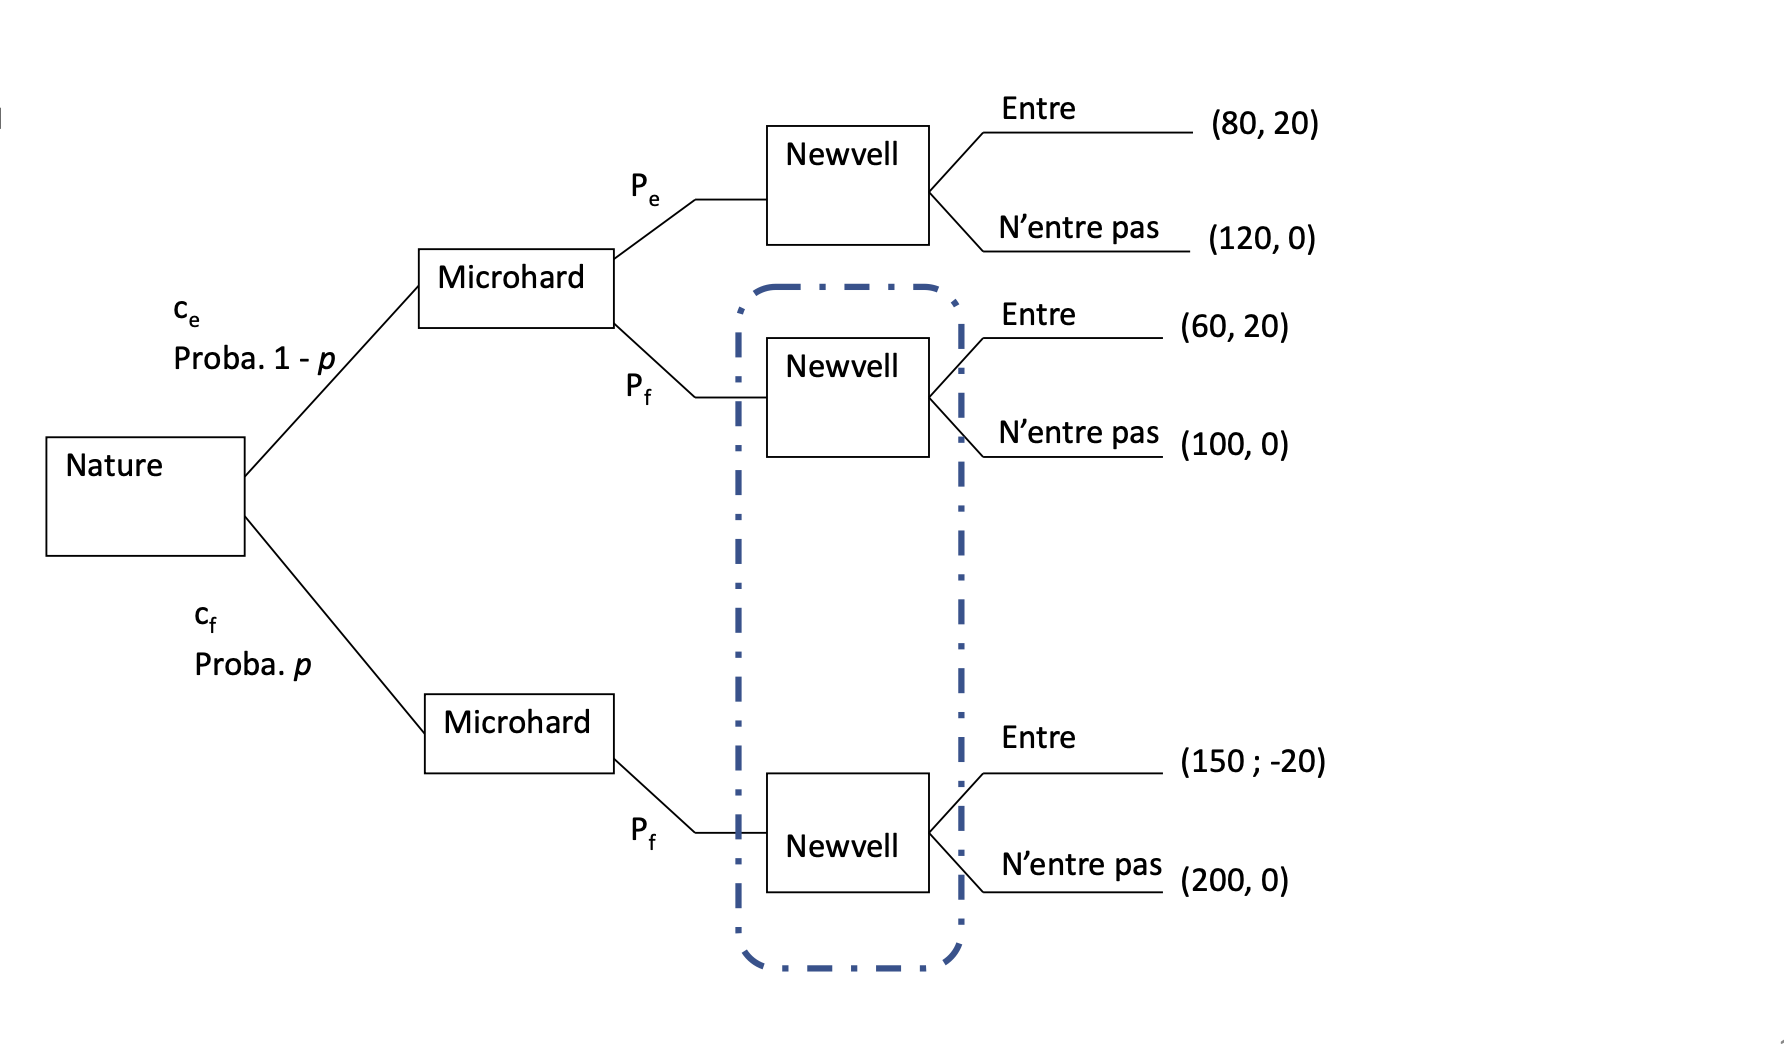
\includegraphics[width=4in]{Arbreq1figAlexis.png}
\end{center}
\end{figure}
\end{frame}  
\begin{frame}
[allowframebreaks]{\insertsection}
\framesubtitle{Question 2: Comportement naïf de Microhard}
\begin{itemize}
  \item Elle ne cherche pas à modifier les incitations de l’entrant en l’informant ou en le désinformant sur ses coûts.
  \item Elle fixe alors en première période le prix de monopole $p_m$
   qui correspond à son niveau 
  de coûts, soit:
  \begin{align*}
    p_m &=\left\{
    \begin{array}{ll}
     p_e &\text{si} \quad c = c_e\\
     p_f &\text{si} \quad c = c_f, \quad \text{avec} \ c_f < c_e, p_f < p_e.
    \end{array}
    \right.
  \end{align*}
  \item Ce faisant, la firme en place révèle son coût à l’entrant qui entre s’il
   observe $p_e$ et n’entre pas s’il observe $p_f$ (donc deux équilibres possibles).
\end{itemize}
\end{frame}  
\begin{frame}
  [allowframebreaks]{\insertsection}
  \framesubtitle{Question 3: Comportement stratégique de Microhard}
  \begin{itemize}
    \item Deux équilibres de Nash (bayésiens)
\begin{enumerate}
  \item Équilibre révélateur:
  \begin{enumerate}[$\cdot$]
    \item Avec cet équilibre, de prime abord, tout se passe donc comme 
    quand la firme en place (Microhard)  se comporte naïvement, 
    à ceci près que la firme en place fixe en première période lorsqu’elle est efficace un prix inférieur à $p_f$ (alors qu’elle fixe $p_e$ lorsque $c = c_e$ ).
    \item La raison en est que la stratégie de la firme en place ne révèle ses coûts que si elle n’a pas intérêt à faire croire à l’entrant qu’elle a un coût faible alors qu’il est élevé.
    \item Il faut donc que signaler un coût faible soit une stratégie coûteuse (trop coûteuse pour qu’une firme inefficace puisse la trouver profitable). Le prix fixé par une firme 
    efficace en première période découle de cette contrainte.
    \item Remarquons que non seulement il n’y a pas de prédation 
    dans l’équilibre révélateur, mais les consommateurs profitent en première période de prix (parfois) plus faibles que quand la firme en place se comporte naïvement, les prix de second période étant quant à eux identiques.
  \end{enumerate}

  \framebreak

  \item Équilibre mélangeant:
  \begin{enumerate}[$\cdot$]
    \item Microhard fixe le même prix en première période quel que soit son coût. 
\item Notons qu’il n’existe pas d’équilibre mélangeant dans lequel l’entrée intervient en seconde période.
\item La raison en est que si tel est le cas, la firme en place a intérêt à maximiser ses profits en première période, donc à fixer le prix de monopole correspondant à ses coûts en première période, ce qui détruit l’équilibre. Les équilibres mélangeant sont donc des équilibres de prédation.
\item En fait, Microhard choisit en première période le prix de monopole correspondant à un coût faible quelle que soit la vraie valeur de son coût. Ce faisant, elle profite des doutes de l’entrant Newvell sur la vraie valeur des coûts, doutes suffisamment forts pour que l’entrée soit empêchée
  \end{enumerate}
\end{enumerate}
  \end{itemize}
\end{frame}  



\begin{frame}
[allowframebreaks]{\insertsection}
\framesubtitle{Question 4: 
Espérance de gains de Newvell si elle rentre alors que Microhard fixe un prix faible}
\begin{itemize}
  \item Si Microhard propose un prix faible en période 1, 
  elle a un coût faible avec un probabilité $\prob$ et un coût élevé avec une probabilité $1 - \prob$. 
  \item En conséquence, son espérance de gains si elle rentre sera de :
\begin{align*}
  20 \times (1 - \prob) - 20 \times \prob = 20 - 20\prob -20\prob = 20 - 40\prob.
\end{align*}
\item N.B. Si Microhard propose un prix élevé en période 1, 
elle a un coût élevé. L’entrée en seconde période rapportera à Newvell un gain certain de 20
\end{itemize}
\end{frame}  
%\begin{frame}[allowframebreaks]{Références}
%\bibliographystyle{jpe}
%\bibliography{../../../Biblio}
%\end{frame}
\begin{frame}
  [allowframebreaks]{\insertsection}
  \framesubtitle{Question 5: 
  On suppose que $\prob> \frac{1}{2}$ et que Newvell le sait. 
  Newvell va-t-elle décider d’entrer ou de ne pas entrer sur le marché ?}
  \begin{itemize}
    \item Si $\prob > \frac{1}{2}$, la probabilité que Microhard ait un coût faible est la plus forte
    \item Dans ce cas l’espérance de gains de Newvell $(20 - 40\prob)$ sera $< 0$. 
    \item En conséquence, elle ne rentrera pas si elle obserbe que Microhard fixe un prix faible.
  \end{itemize}
\end{frame}  
\end{document}
